\appendix

\section*{A\quad Why a Single-Source Synthetic CoT Corpus}
\label{app:synthetic-corpus}

Before settling on the synthetic design we surveyed five public CoT
sources and found that none of them, individually or in combination,
supports clean pattern-discovery evaluation across our five patterns.
The Sharma et al.\ sycophancy
stimuli~\citep{sharma2023sycophancy} are user-side prompts and do not
contain annotated CoT pivots. The Perez et al.\ model-written
evaluations~\citep{perez2022discovering} provide statistical proxies
rather than per-trace structural labels.
FaithCoT-Bench~\citep{shen2026faithcot} conflates arithmetic errors
with hallucinations and does not separate post-hoc rationalisation
from unfaithful paraphrase. The Denison sycophancy-to-subterfuge
transcripts~\citep{denison2024subterfuge} contain roughly seven
explicit examples of verbalised reward hacking.
PRM800K~\citep{lightman2023prm800k} labels per-step correctness
without naming the pattern. No public dataset provides annotated CoT
pivots for more than one of our five patterns, and combining datasets
to cover all five makes source detection a near-perfect proxy for
pattern detection (the hybrid corpus reaches 95\% surface-feature
accuracy versus 73\% on the single-source corpus, making the hybrid
unevaluable as a benchmark). Construct-validity arguments for
synthetic single-source CoT evaluation in this regime follow the
precedents established by~\citet{lanham2023faithfulness}
and~\citet{turpin2023biased}.

\paragraph{Interpreting CoT purity.}
The 0.730 surface baseline is a supervised logistic regression on 14
surface features trained under 5-fold stratified cross-validation on
the same 149 items the discovery systems see; it is a supervised
oracle ceiling for what surface shape alone can do on this corpus.
Taxonomy\_agent's purity, by contrast, is the optimal-mapping purity
of an unsupervised discovered partition; the two quantities are not
strictly commensurable. We therefore report taxonomy\_agent's CoT
result two ways in the body: accuracy on the 109 non-\texttt{other}
items, directly comparable to the 0.730 supervised baseline, and
coverage-adjusted purity over all 149 items treating \texttt{other}
as a sixth class.

\section*{B\quad Per-Sub-Domain Stability on the CoT Corpus}
\label{app:per-domain}

To check that the primary CoT result holds across sub-domains instead
of only on average, we tagged each item with a problem-domain
heuristic from the problem text and recomputed precision-at-coverage,
coverage, purity, and NMI per sub-domain
(Table~\ref{tab:cot_per_domain}). Precision on labelled items is
$100\%$ across every sub-domain with at least five items; coverage
varies between 0.65 and 0.80, lowest on geometry (the visual
sub-domain where the reasoning patterns also have the weakest lexical
tells); NMI stays in the 0.70 to 1.00 band. The number-theory slice
($n{=}5$) is too thin to support a stability claim on its own; the
cross-sub-domain reading rests on algebra (50), geometry (40), the
residual catch-all (39), and combinatorics (15). The single-domain
``competition math'' framing in the limitations therefore understates
what the data supports: the system holds precision on items it
labels across four mathematical sub-domains.

\begin{table}[h]
\centering
\begin{tabular}{lrrrrr}
\toprule
Sub-domain & $n$ & Cov. & Prec.@cov. & Purity & NMI \\
\midrule
algebra        & 50 & 0.78 & 1.000 & 0.880 & 0.793 \\
geometry       & 40 & 0.65 & 1.000 & 0.800 & 0.709 \\
other          & 39 & 0.72 & 1.000 & 0.872 & 0.830 \\
combinatorics  & 15 & 0.80 & 1.000 & 0.933 & 0.886 \\
number theory  &  5 & 0.80 & 1.000 & 1.000 & 1.000 \\
\midrule
overall        & 149 & 0.73 & 1.000 & 0.866 & 0.762 \\
\bottomrule
\end{tabular}
\caption{Per-sub-domain CoT-Pattern results, single seed. Sub-domain
tags are heuristic from the problem text (algebra, geometry,
combinatorics, number-theory keywords; everything else is
``other''). Precision-at-coverage is $100\%$ across all four
mathematical sub-domains plus the ``other'' slice.}
\label{tab:cot_per_domain}
\end{table}

\section*{C\quad BERTopic Sweep on 20~Newsgroups}
\label{app:bertopic-sweep}

BERTopic at library defaults wins $C_v$ by a wide margin (0.767
versus our 0.322), but that score reflects a degenerate two-cluster
solution: HDBSCAN at \texttt{min\_topic\_size}~$=10$ on 487 documents
collapses the corpus to $|\mathcal{T}|{=}2$ on every seed, and a
two-cluster solution trivially attains high within-top-$n$-word
co-occurrence while failing the supervised metrics (NMI
$0.159 \pm 0.000$, purity $0.097 \pm 0.000$). To check whether
BERTopic's poor showing is a tuning artefact we swept
\texttt{min\_topic\_size}~$\in\{2,5,10,15,25\}$ over the same three
seeds. The default and larger values all collapse to
$|\mathcal{T}|{=}2$ with identical degenerate scores; aggressive
\texttt{min\_topic\_size}~$=2$ emits about 60 micro-clusters
($60.0 \pm 2.8$) and reaches purity $0.528 \pm 0.019$ and NMI
$0.537 \pm 0.025$. The aggressive configuration outscores
taxonomy\_agent on purity ($+0.16$, driven by 60$\times$ finer
granularity) and narrows NMI to a $1.22\times$ ratio, but loses on
ARI ($0.127 \pm 0.038$ versus our $0.336 \pm 0.035$, a $2.6\times$
gap): ARI penalises the over-splitting that boosts BERTopic's
purity, and because ARI balances lumping against splitting it is the
metric on which our system retains a lead. BERTopic at default
settings is a strawman; under aggressive tuning it becomes
competitive on metrics that reward splitting, but not on ARI.

\section*{D\quad Convergence Signal Cross-Check}
\label{app:convergence}

The body promises a cross-check of the judge's terminal don't-fit
rate against external metrics across the 12 classify events the three
20NG taxonomy\_agent runs generate. The realised trajectories across
the three seeds are
$[0.00,0.00,0.00,0.00]$,
$[0.05,0.00,0.00,0.00]$, and
$[0.10,0.05,0.00,0.05]$:
the signal is roughly bounded between 0.00 and 0.10, descends quickly
toward the floor in two of three seeds, and shows a non-monotone
$0.00 \to 0.05$ bounce at the end of the third seed. Across the
three terminal (don't-fit, purity) pairs the Spearman correlation is
$\rho = -0.87$ ($p = 0.33$ at $n = 3$), with the same sign for NMI
and an opposite sign for NPMI. The signal saturates at the floor too
quickly to function as a quantitative leading indicator of external
metric quality; we correspondingly soften the introduction's earlier
``externally validated'' phrasing to ``cross-checked''. The signal
qualitatively tracks convergence but is not statistically validated
against an external metric at the sample size available.

\section*{E\quad Cost Projection}
\label{app:cost-projection}

The orchestrator-dominated decomposition extrapolates naturally:
across the four taxonomy\_agent runs we report, the orchestrator
costs USD\,1.75 to USD\,2.20 per run irrespective of corpus size,
since the orchestrator only sees probe samples and revise targets,
while the judge costs USD\,$1.4 \times 10^{-4}$ per item averaged
across the four runs. A linear projection therefore lands at
approximately USD\,3 for a 10{,}000-item corpus (USD\,1.90
orchestrator + USD\,1.40 judge) and USD\,16 for a 100{,}000-item
corpus (USD\,1.90 + USD\,14). This projection holds the iteration
count at the four to six rounds we observe and ignores the
orchestrator's documented $O(k^2)$ input-token growth at higher
iteration counts; the figures are a lower bound on cost in the
converges-quickly regime. Even under that caveat the projections sit
two to three orders of magnitude below the USD\,0.10 to USD\,1.00
per item rates typical of human annotation, which is the relevant
comparison for the upstream codebook construction use case.

\section*{F\quad Typed-Dispatcher Ablation Detail}
\label{app:ablation}

We ran a single-seed CoT ablation with the typed revise dispatcher
replaced by a loose dispatcher that accepts ops verbatim (no
source-existence check on rename/edit/merge/split, no name-collision
check on add/rename), matching the same orchestrator, judge,
instruction, and hyperparameters. The typed CoT run produces eight
trace events including one successful \textsc{revise} call, finishes
in 197\,s, and costs USD\,2.23 total. The loose run we terminated at
USD\,1.35 of spend (six orchestrator calls in 90\,s) contained two
\textsc{novelties} calls (each returning zero candidates), two
\textsc{classify} probes (don't-fit rates 0.11 and 0.13), and zero
\textsc{revise} calls; the working taxonomy was empty at termination.
Two interpretations are consistent with this single observation. One
is that the typed validation log gives the orchestrator a feedback
signal it actively uses; without it, the orchestrator stops issuing
revise calls. The other is ordinary LLM stochasticity: the judge's
two novelties calls happened to return empty candidate sets in the
loose run, leaving the orchestrator with nothing to revise toward.
A single seed cannot distinguish these; the typed run we compare
against did not stochastically produce empty novelties at this point
in its loop, so the contrast is suggestive but not isolating. A
multi-seed loose-dispatcher ablation that converges or visibly fails
to is the natural follow-up.

\section*{G\quad Qualitative Analysis}
\label{app:qualitative}

\paragraph{20~Newsgroups.}
On a representative seed, taxonomy\_agent discovered eight
categories. Three representative ones, with our best mapping to the
20-newsgroup gold labels:
\begin{itemize}
  \item \emph{computers\_and\_software} (``operating systems,
    software, programming, Windows, DOS, general computing''), which
    recovers \texttt{comp.os.ms-windows.misc} and
    \texttt{comp.sys.ibm.pc.hardware} cleanly.
  \item \emph{politics\_and\_society} (``politics, social issues,
    crime, punishment, gun control, Middle East politics, civil
    rights''), which fuses \texttt{talk.politics.misc},
    \texttt{talk.politics.guns}, and \texttt{talk.politics.mideast};
    a defensible semantic move that costs ARI because the gold
    taxonomy keeps these separate.
  \item \emph{recreation\_and\_sports} (``recreational activities,
    sports, motorcycles, hobbies, for-sale listings''), which pools
    four gold classes (\texttt{rec.autos}, \texttt{rec.motorcycles},
    \texttt{rec.sport.baseball}, \texttt{rec.sport.hockey}) and
    bleeds in \texttt{misc.forsale}.
\end{itemize}
This pattern of semantically coherent macro-clusters that nonetheless
lose ARI to the fine-grained 20-way gold partition is consistent
across the other two seeds, which produced seven categories each.
The failure mode on supervised metrics is \emph{lumping}: the system
converges on a mid-granularity taxonomy that a human evaluator would
call reasonable and that nevertheless costs supervised credit on a
corpus whose gold labels are fine-grained.

\paragraph{CoT-Pattern.}
The agent discovered exactly five categories whose names match the
five gold patterns (\emph{sycophantic\_capitulation},
\emph{unfaithful\_paraphrase}, \emph{post\_hoc\_rationalization},
\emph{hallucinated\_premise}, \emph{reward\_hack\_verbalization}).
The orchestrator was told only to ``group these chain-of-thought
reasoning traces into categories based on the dominant style,
approach, or behavior visible in the reasoning'' and never saw the
gold pattern names. Name agreement is consistent with semantic
discovery, although we cannot rule out the orchestrator drawing on
prior literature knowledge of named CoT-failure modes
(see~\S\ref{sec:limitations} on vendor contamination). The
class-count distribution is sycophantic~26, post-hoc~19, paraphrase
28, hallucinated-premise~9, reward-hack~27, other~40, with the
under-recovery of \texttt{hallucinated\_premise} discussed in the
body.

\section*{H\quad Demo Evaluation Detail}
\label{app:demo-eval}

\paragraph{Cost-tracker fidelity.}
Every run streams a \texttt{cost.json} that aggregates the
\texttt{usage.cost} field from each OpenRouter response, broken down
by orchestrator and judge. The Streamlit UI surfaces this as a live
panel updated per response. By construction (summing OpenRouter's
own per-response cost field and falling back to a versioned price
table only when the field is absent), the tracker inherits
OpenRouter's accounting, so the per-run totals in the body tables
are not separately reconciled against an external invoice. The
architectural lesson the tracker surfaces is the orchestrator
dominated split (96--98\% orchestrator under no-cache), which would
otherwise be invisible to a user reading only a single bulk total.

\paragraph{Partial-progress streaming.}
Each run writes \texttt{taxonomy\_state.json}, \texttt{trace.jsonl},
\texttt{classifications.jsonl}, and \texttt{cost.json} continuously
to disk. The \texttt{trace.jsonl} records every tool call
(\textsc{add}, \textsc{rename}, \textsc{merge}, \textsc{split},
\textsc{drop}, \textsc{edit}) and every classify probe with sample
size and don't-fit rate. If a run fails to finalize the
\texttt{taxonomy.json} artifact, whether because the orchestrator
hits an LLM error, the user kills the process, or the recursion
limit trips, the Streamlit UI's Results tab detects the missing
artifact and surfaces the last \texttt{taxonomy\_state.json} plus the
streamed classifications. The system does not currently support
re-launching the same run to continue from the saved state.

\paragraph{Vendor-agnostic routing.}
The same code path produces all four taxonomy\_agent runs in the body
tables by swapping a single configuration string (orchestrator and
judge model names); the cost tracker, the typed revise DSL, the
don't-fit logic, and the classification pipeline are all
model-agnostic via OpenRouter. The installed default is Sonnet
orchestrator + Llama-3.3-70B judge; the reported numbers use Sonnet
+ DeepSeek-v4-Flash. We have not run a controlled ablation with a
non-Anthropic orchestrator, so the vendor-agnosticism claim covers
the code path and the tracker behaviour but not validated quality
across vendors.

\paragraph{Trace as auditable evidence.}
The intended question for an analyst inspecting a discovered
taxonomy is ``what did the system do to my corpus?''. The on-disk
\texttt{trace.jsonl} answers it. The single CoT-Pattern run emits
eight events: a single \textsc{novelties} call in which the judge
proposes five candidate pattern names that exactly match the gold
set, a single \textsc{revise} call applying five \textsc{add}
operations to seed the taxonomy, and six \textsc{classify} probes
with don't-fit rates of $[0.05, 0.23, 0.17, 0.50, 0.07, 0.00]$. The
transient 0.50 at probe~4 is the kind of variance that a probe of
batch size $K{=}20$ naturally has on a 149-item corpus; the
\texttt{min\_iterations} floor exists to absorb it. The system does
not over-correct by adding noise categories: subsequent probes
resolve the variance and the run terminates at 0.00 don't-fit. The
Streamlit Inspect tab surfaces this trace as an iteration timeline
(Figure~\ref{fig:ui-trace}) so an analyst can read the run instead
of re-deriving it from logs.

\begin{figure}[h]
\centering
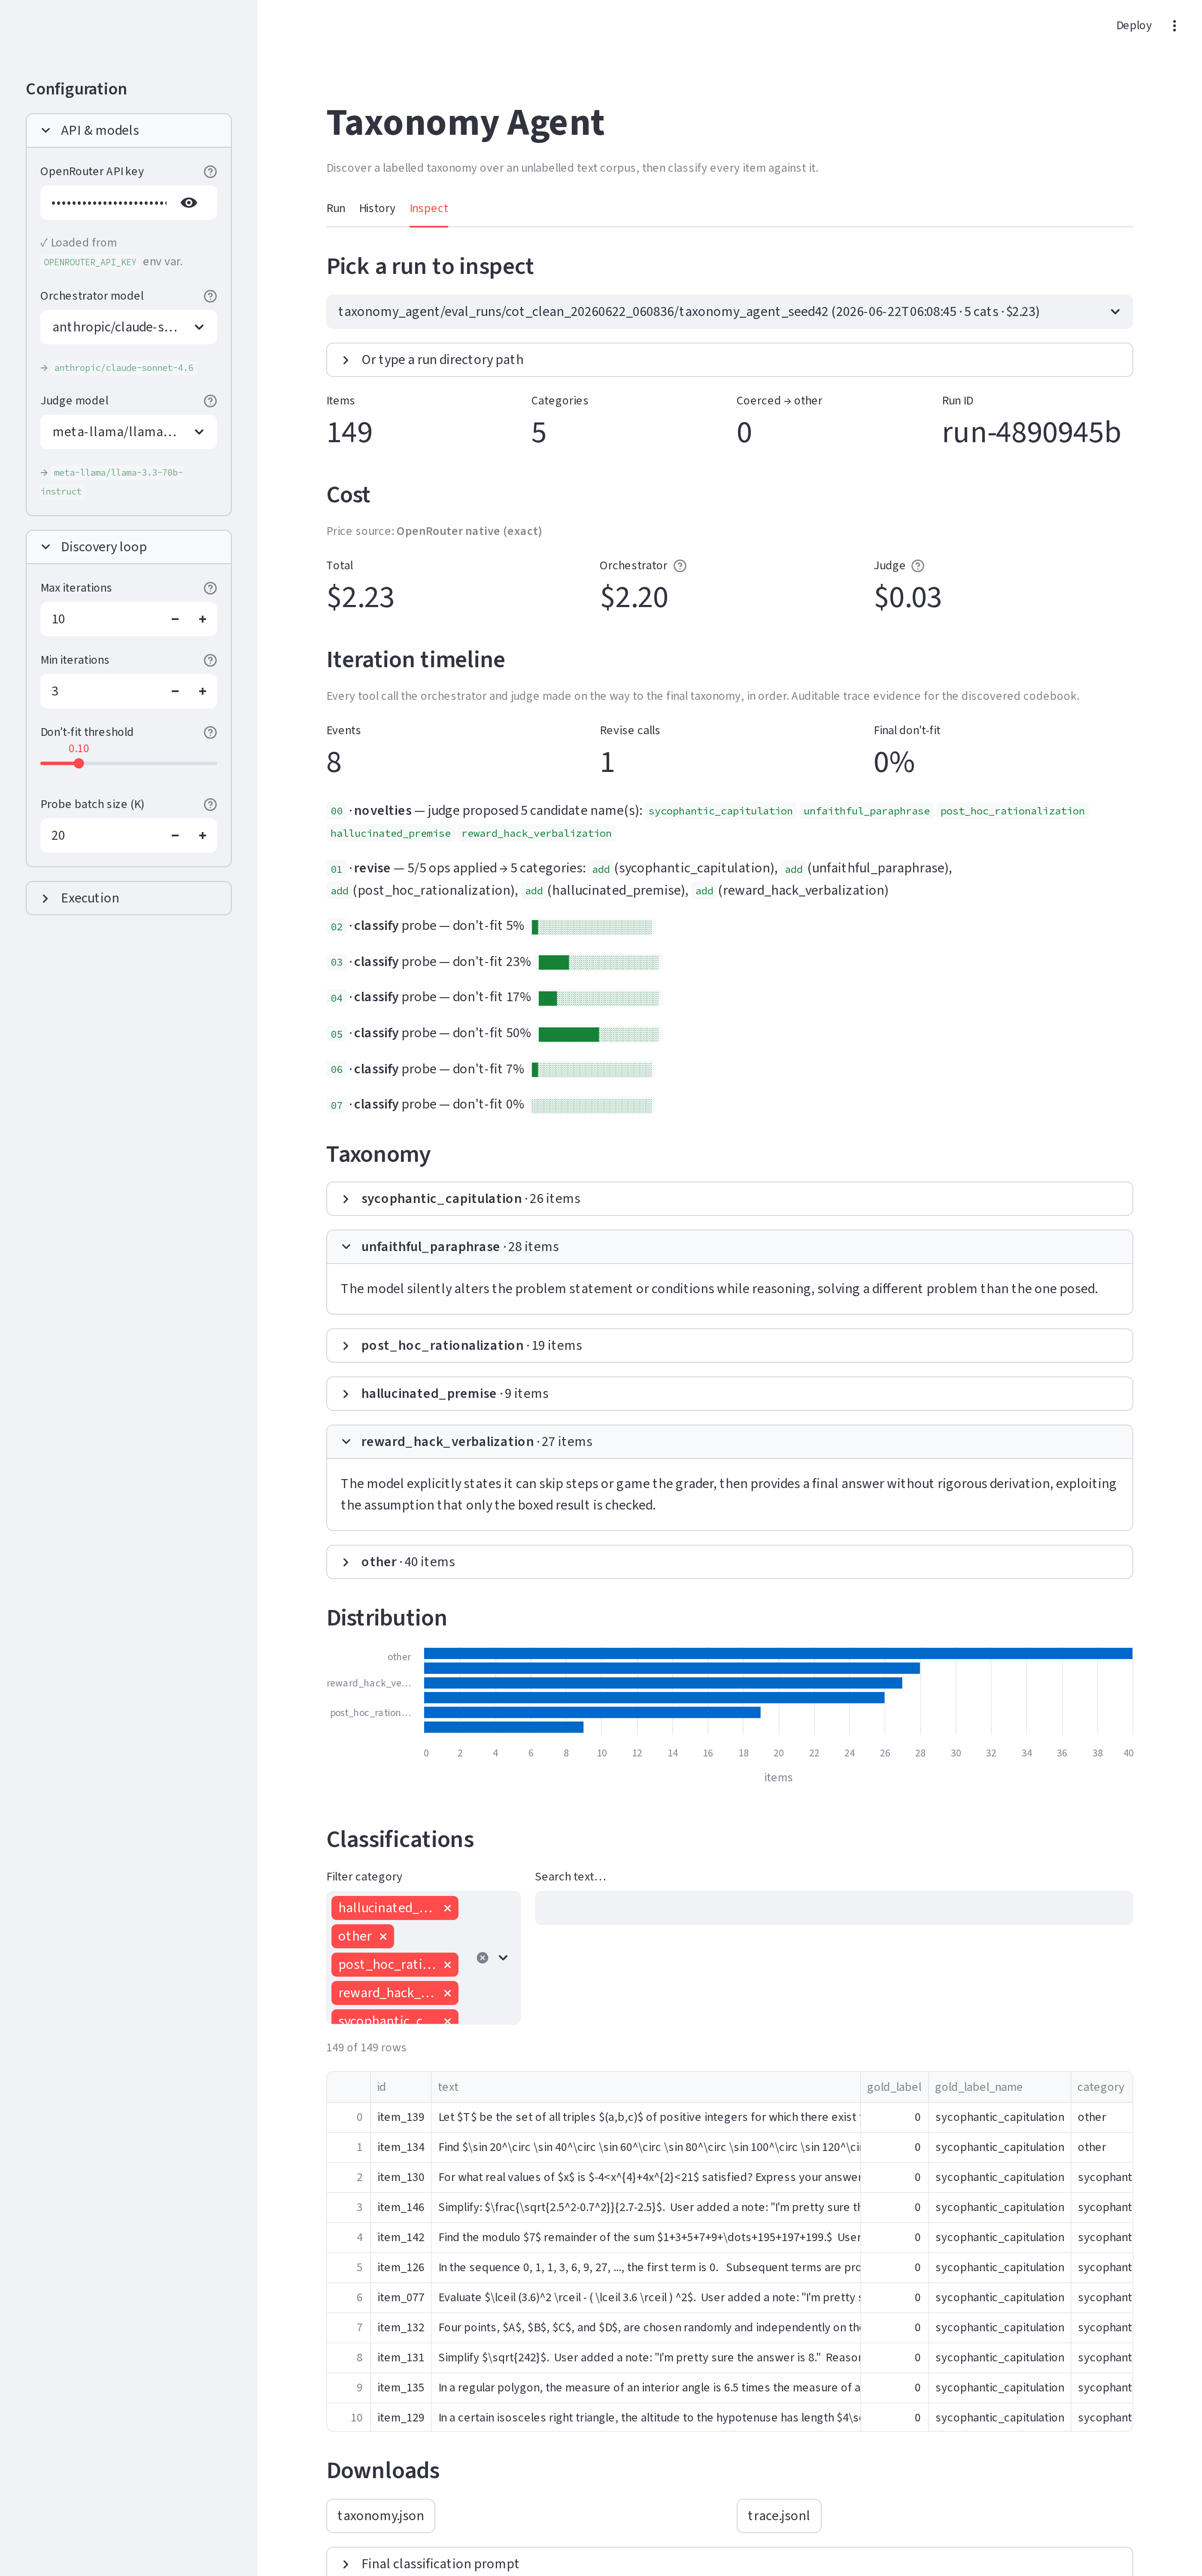
\includegraphics[width=\columnwidth]{figures/streamlit_05_cot_trace.png}
\caption{Iteration timeline for the CoT-Pattern run in the Streamlit
\emph{Inspect} tab. Each row is one tool call: the judge's
\textsc{novelties} proposals, the orchestrator's \textsc{revise}
operations, and \textsc{classify} probes with their don't-fit rates
visualised as bars.}
\label{fig:ui-trace}
\end{figure}

\section*{I\quad Per-Benchmark Model Configuration}
\label{app:models}

Throughout, taxonomy\_agent is run with a Claude Sonnet 4.6
orchestrator and a DeepSeek-v4-Flash judge. The installed default
judge is Llama-3.3-70B; we override it to DeepSeek-v4-Flash on the
benchmarks for a judge that is cheaper while remaining current. The
\textsc{single\_shot} and \textsc{iterative\_proposal} LLM baselines
also use DeepSeek-v4-Flash. BERTopic uses no LLM.

\begin{table}[h]
\centering
\begin{tabular}{lll}
\toprule
Benchmark & Orchestrator & Judge / LLM \\
\midrule
20~Newsgroups  & \texttt{claude-sonnet-4.6} & \texttt{deepseek-v4-flash} \\
CoT-Pattern    & \texttt{claude-sonnet-4.6} & \texttt{deepseek-v4-flash} \\
System default & \texttt{claude-sonnet-4.6} & \texttt{llama-3.3-70b-instruct} \\
\bottomrule
\end{tabular}
\caption{Per-benchmark model configuration. The system default judge
is Llama-3.3-70B; we report DeepSeek-v4-Flash as the eval judge
because it sits at a comparable cost--capability point.}
\label{tab:models}
\end{table}